\subsection{Inventory management}
The sequence diagram represented in figure \ref{3img:[sequence]inventory}
describes the procedure needed for inserting or remove an item from the
inventory.

The item is added or removed from the budget of the project who needs it,
in this way is possible to monitor and give a measure of the cost of each
project.

The user who modifies the inventory has to be authenticated, checking if
he has the permission to operate on that specific resource.

\begin{figure}[H]
\begin{centering}
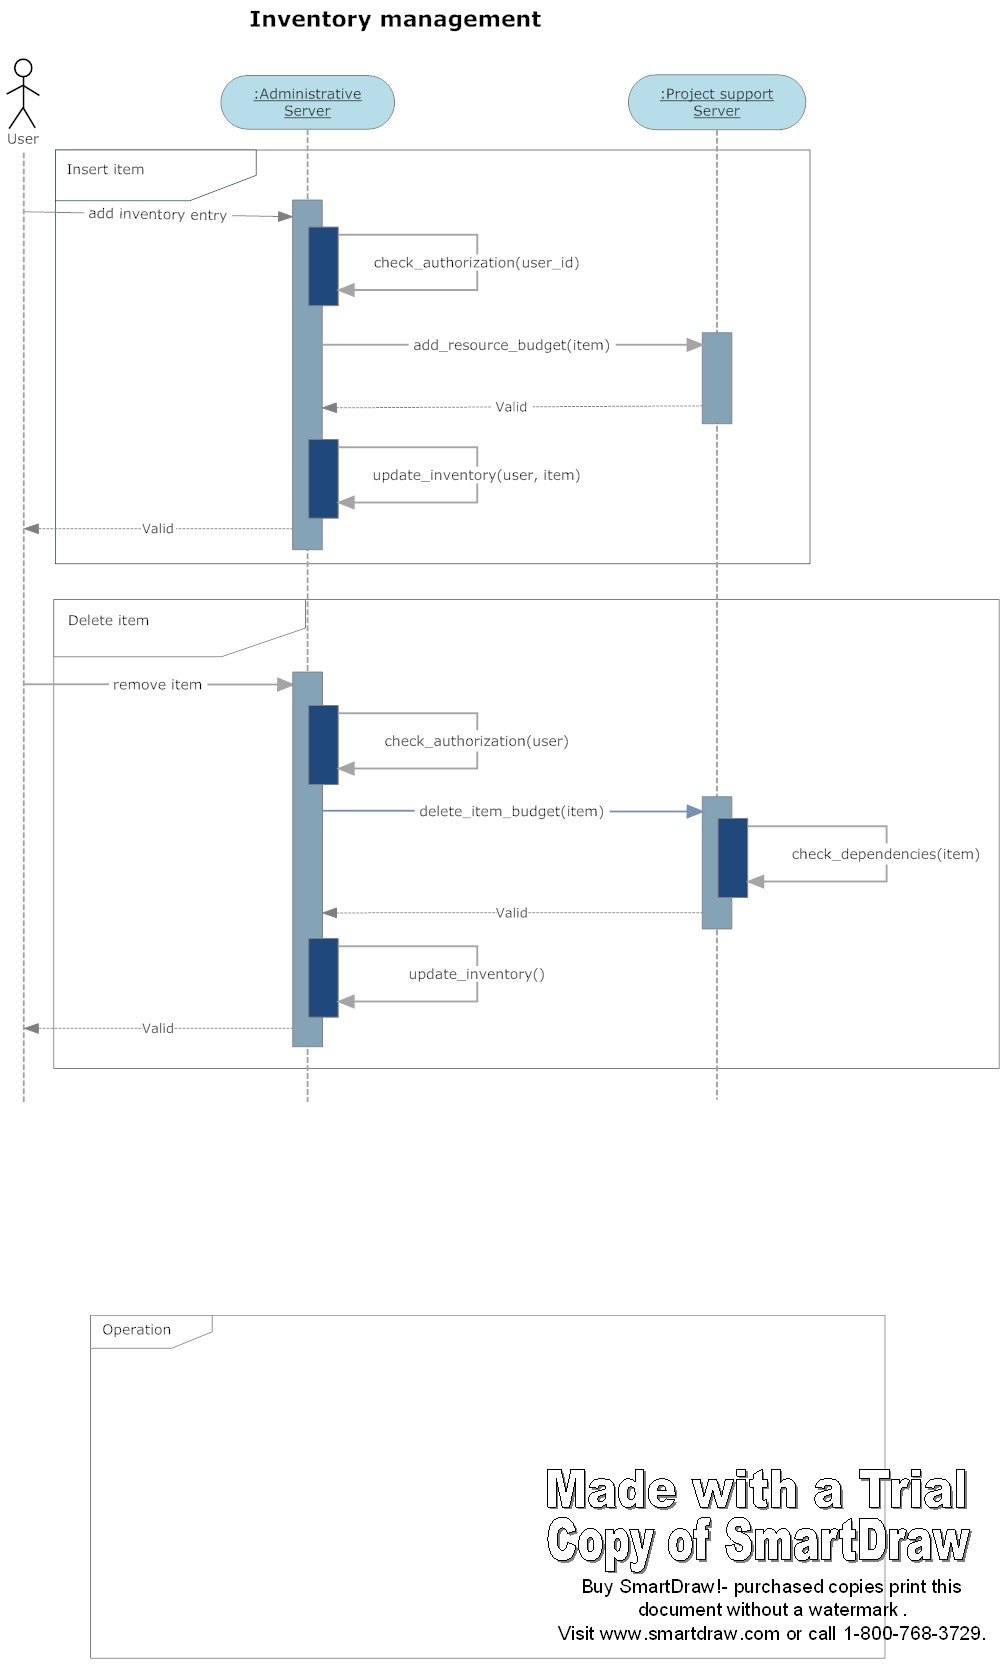
\includegraphics[scale=0.45]{assign3/sdraw/imgs/inventory.jpg}
\caption{Inventory management sequence diagram.}
\label{3img:[sequence]inventory}
\end{centering}
\end{figure}
